\section{Experiments}
\label{sec:experiments}


In this section, we report a series of experiments in which
we explore the kinds of linguistic regularities the networks learn from
word-level input.
In Section~\ref{sec:computeomission} we introduce \emph{omission score},
a metric to measure the contribution of each token to the prediction
of the networks, and in Section~\ref{sec:omitimaginet} we analyze how
omission scores are distributed over dependency relations and
part-of-speech categories.
In Section~\ref{sec:beyondlexical} we investigate the extent to which
the importance of words for the different networks depend on the words themselves,
their sequential position, and their grammatical function in the sentences.
Finally, in Section~\ref{sec:contexts} we systematically compare the types of
n-gram contexts that trigger individual dimensions in the hidden layers of the
networks, and discuss their level of abstractness.

In all these experiments we report our findings based on the {\sc Imaginet}
model, and whenever appropriate compare it to our two other models {\sc LM} and {\sc Sum}.
For all the experiments, we trained the models on the training portion of the
MSCOCO image-caption dataset \citep{lin2014microsoft}, and analyzed the
representations of the sentences in the validation set corresponding
to 5000 randomly chosen images. The target image representations were
extracted from the pre-softmax layer of the 16-layer CNN of
\cite{simonyan2014very}.



\begin{figure*}[t]
  \centering
  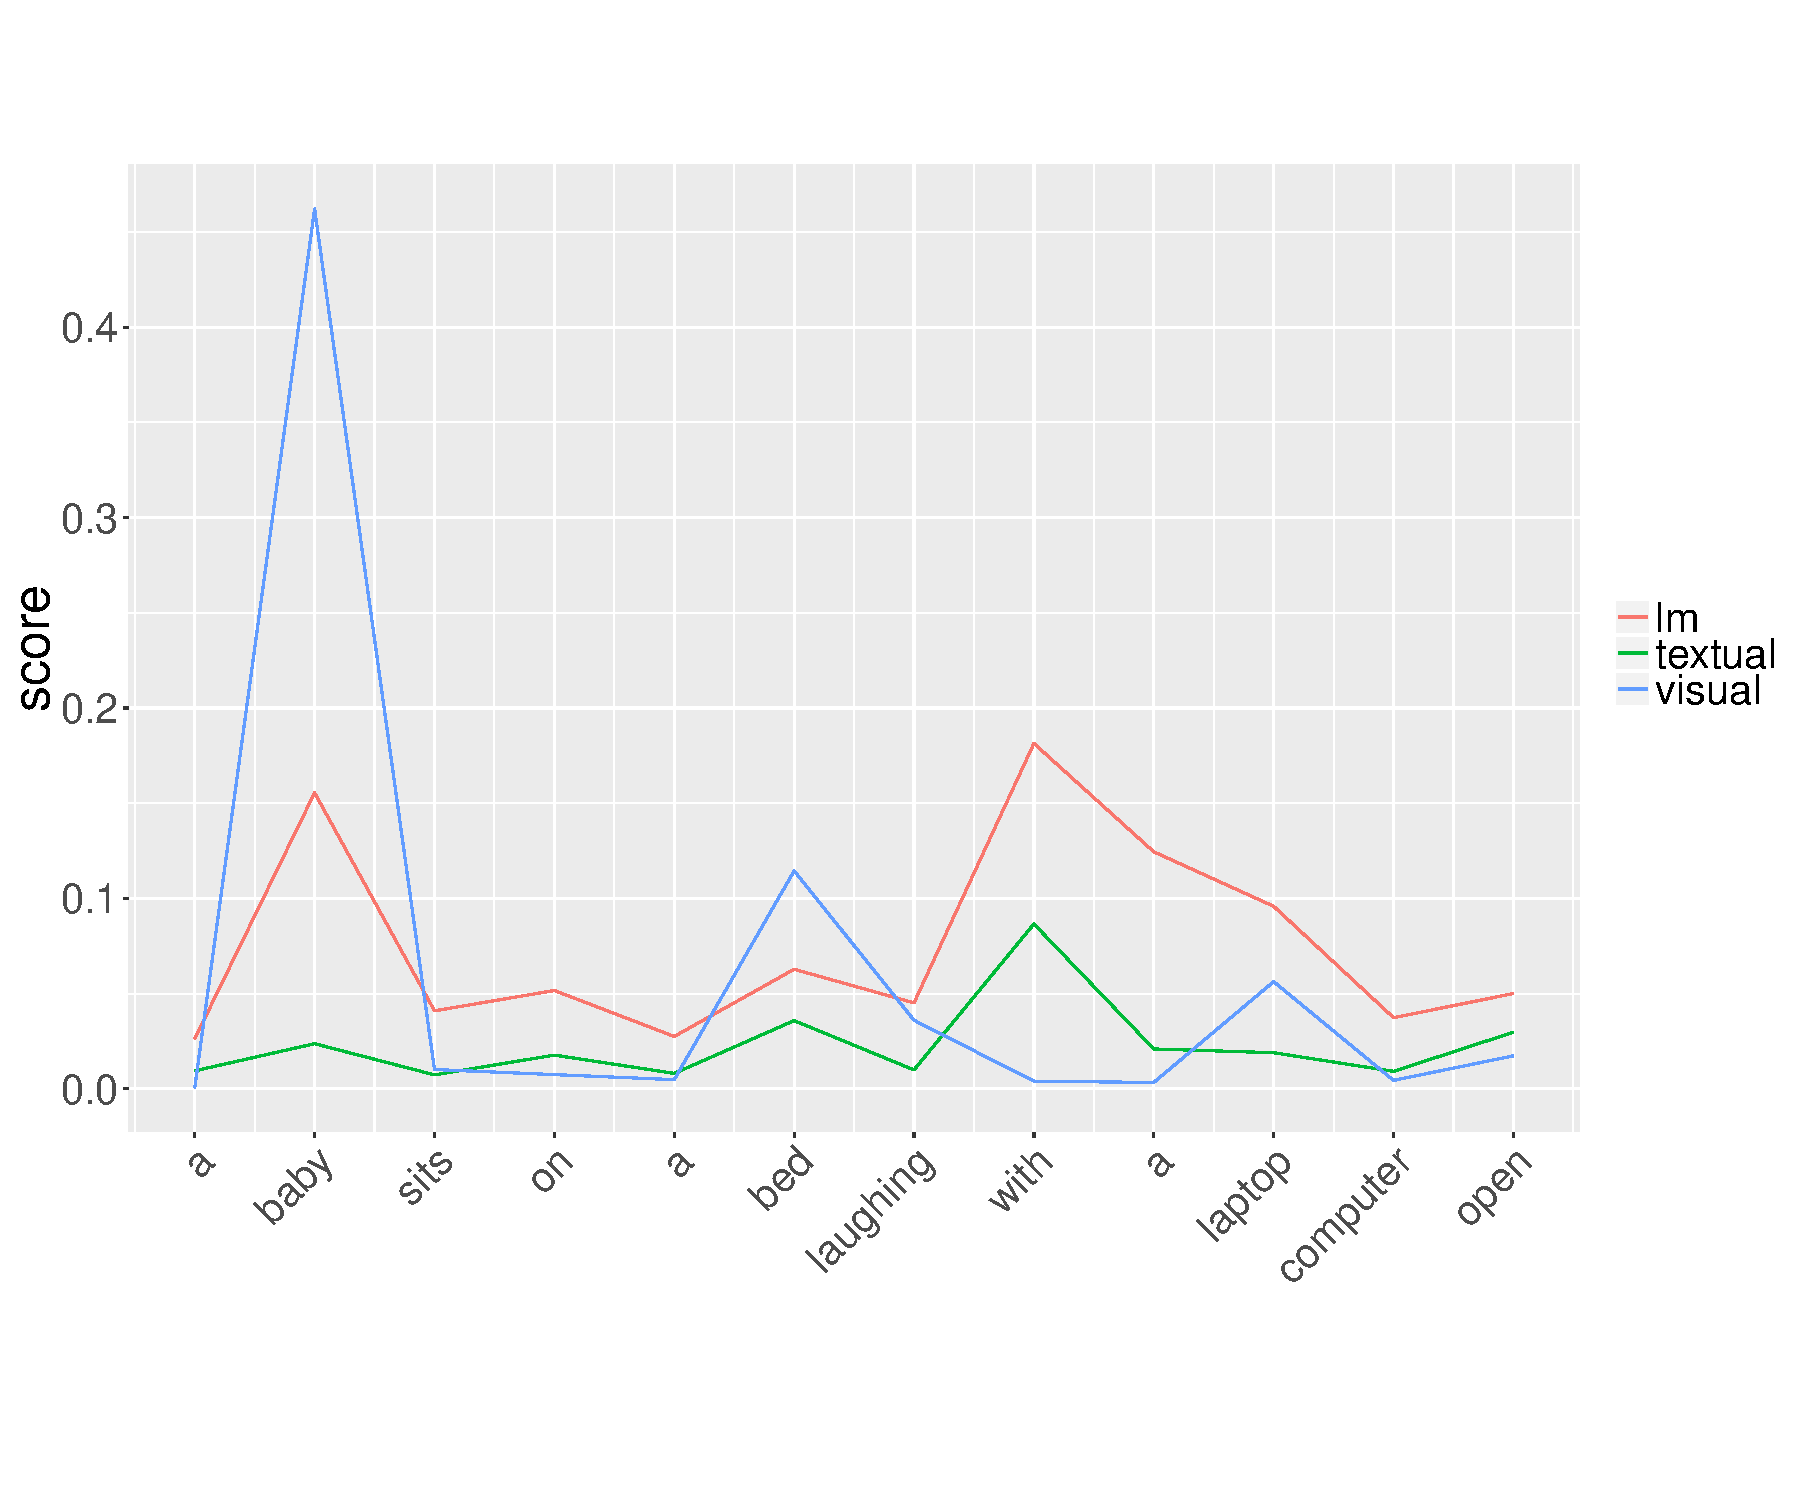
\includegraphics[scale=0.3]{chapters/COLI/omissionex.pdf}
  \caption{Omission scores for the example sentence {\it a baby sits
      on a bed laughing with a laptop computer open} for {\sc LM} and
    the two pathways, {\sc Textual} and {\sc Visual}, of {\sc
      Imaginet.}}
  \label{fig:omissionex}
\end{figure*}

\begin{figure*}[t]
  \centering
  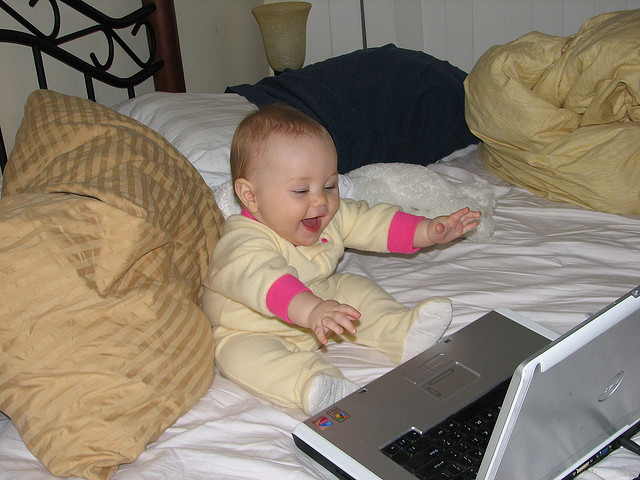
\includegraphics[scale=0.25]{chapters/COLI/85826.jpg}
  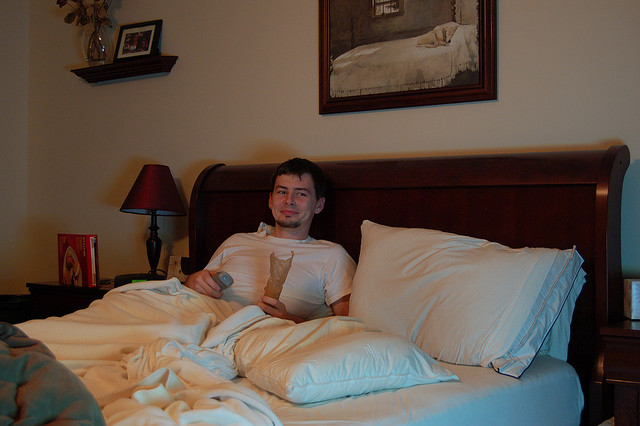
\includegraphics[scale=0.25]{chapters/COLI/60596.jpg}
  \caption{Images retrieved for the example sentence {\it a baby sits
      on a bed laughing with a laptop computer open} (left) and the
    same sentence with the second word omitted (right).}
  \label{fig:omissionexpic}
\end{figure*}



\subsection{Computing Omission Scores}
\label{sec:computeomission}

We propose a novel technique for interpreting the
activation patterns of neural networks trained on language tasks
from a linguistic point of view, and focus
on the high-level understanding of what parts of the input sentence the networks
pay most attention to. Furthermore, we investigate if the networks
learn to assign different amounts of importance to tokens depending
on their position and grammatical function in the sentences.\label{edit:whyposdep}

In all the models the full sentences are represented by the
activation vector at the end-of-sentence symbol
($\mathbf{h}_\text{end}$). We measure the salience of each word $S_i$
in an input sentence $S_{1:n}$ based on how much the representation of the
partial sentence $S_{\setminus i} = S_{1:i-1}S_{i+1:n}$, with
the omitted word $S_i$, deviates from that of the original sentence
representation. For example, the distance
between $\mathbf{h}_\text{end}($``{\it the black dog is running}''$)$
and $\mathbf{h}_\text{end}($``{\it the dog is running}''$)$ determines
the importance of {\it black} in the first sentence. We introduce the
measure $\mathrm{omission}(i,S)$ for estimating the salience of a word $S_i$:

\begin{equation}
\label{eg:omit}
\mathrm{omission}(i,S) = 1-\mathrm{cosine}(\mathbf{h}_\text{end}(S),
\mathbf{h}_\text{end}(S_{\setminus i}))
\end{equation}

Figure~\ref{fig:omissionex} demonstrates the omission
scores for the {\sc LM}, {\sc Visual} and {\sc Textual} models for an
example caption.
Figure~\ref{fig:omissionexpic} shows the images retrieved by {\sc
  Visual} for the full
caption and for the one with the word {\it baby} omitted.
The images are retrieved from the validation set of MS-COCO by: 1)
computing the image representation of the given sentence with {\sc
  Visual}; 2) extracting the CNN features for the images from the set;
and 3) finding the image that minimizes the cosine distance to the
query.\label{edit:retrievalexplain}
The omission scores for {\sc Visual} show that the model paid attention
mostly to {\it baby} and {\it bed} and slightly to {\it laptop}, and
retrieved an image depicting a baby sitting on a bed with a laptop.
Removing the word {\it baby} leads to an image that depicts an adult
male laying on a bed. Figure~\ref{fig:omissionex} also shows that in
contrast to {\sc Visual}, {\sc Textual} distributes
its attention more evenly across time steps instead of focusing on the
types of words related to the corresponding visual scene. The peaks
for {\sc LM} are the same as for {\sc Textual}, but the variance of
the omission scores is higher, suggesting that the unimodal language
model is more sensitive overall to input perturbations than {\sc Textual}.




%-----------------
\subsection{Omission score distributions}
\label{sec:omitimaginet}


%-----------------
\label{subsec:omission-text-vis}
\begin{figure}[!htbp]
\centering
\hspace*{-0.3in}
\setlength{\tabcolsep}{0pt}
\begin{tabular}{cc}
  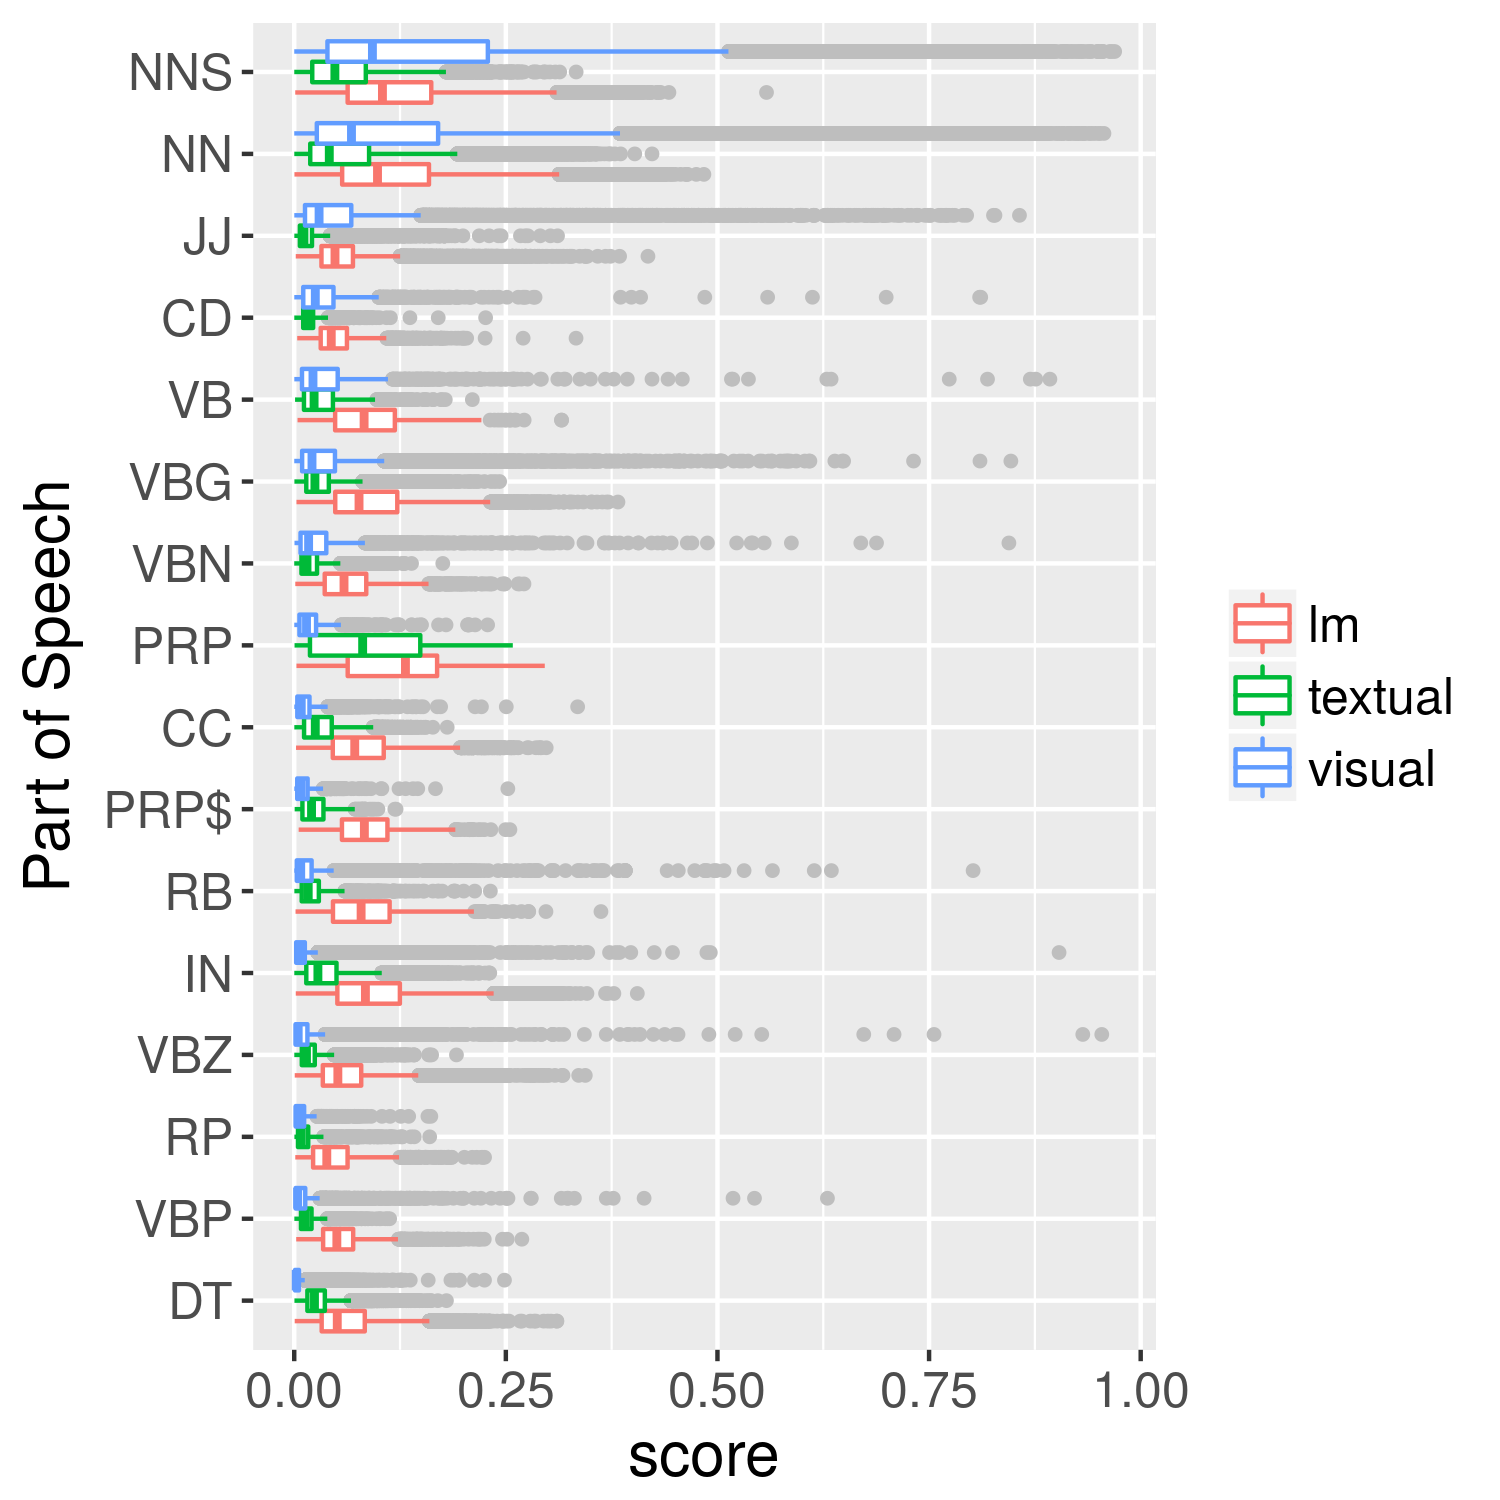
\includegraphics[scale=0.5]{chapters/COLI/imaginet-omission-pos-boxplot.png}
	&
  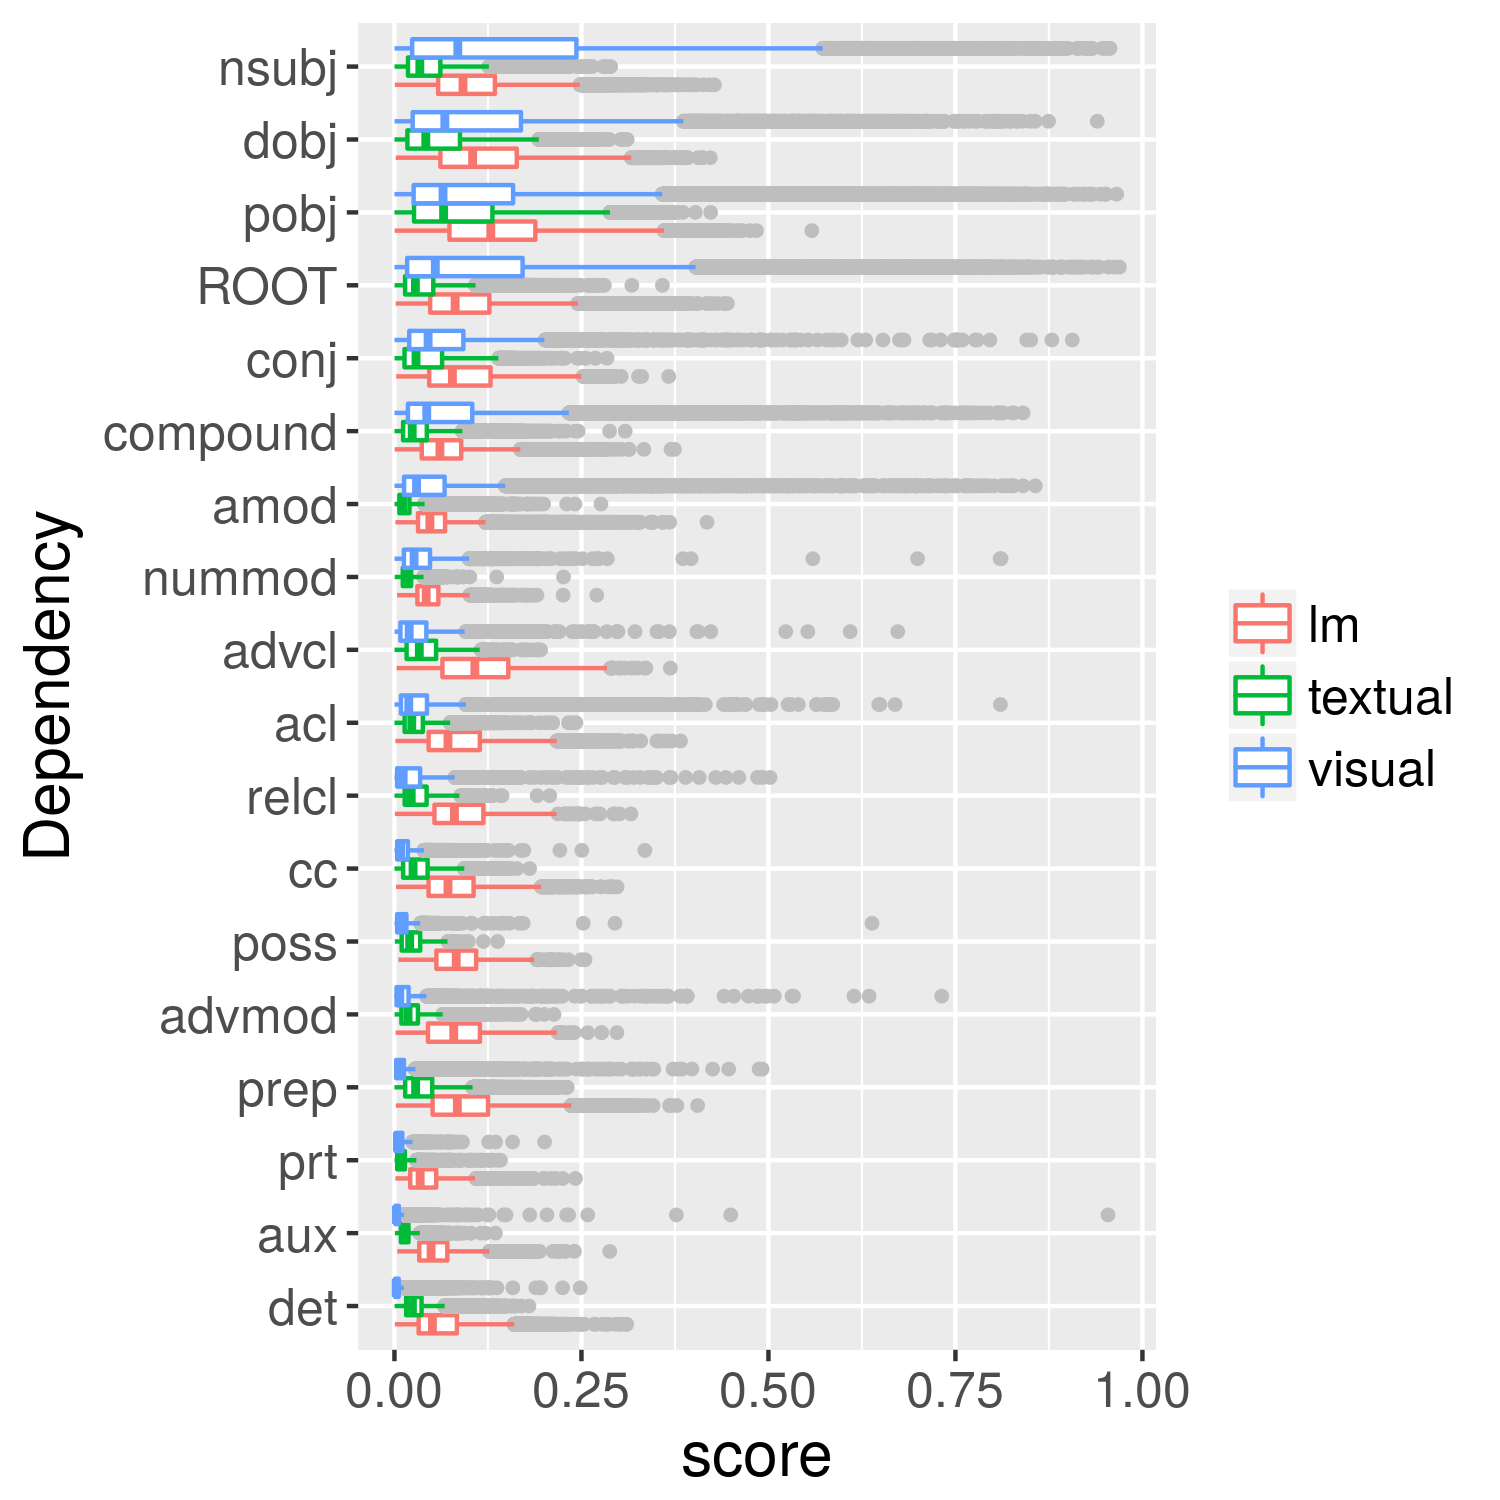
\includegraphics[scale=0.5]{chapters/COLI/imaginet-omission-dep-boxplot.png}
  \end{tabular}

\caption{Distribution of omission scores for POS (left) and dependency labels
  (right), for the {\sc Textual} and {\sc Visual} pathways and for
  {\sc LM}. Only labels which occur at least 1250 times are included.}
\label{fig:omission-imaginet}
\end{figure}

\begin{figure*}[t]
  \centering
  \hspace*{-0.2in}
  \setlength{\tabcolsep}{0pt}
  \begin{tabular}{cc}
  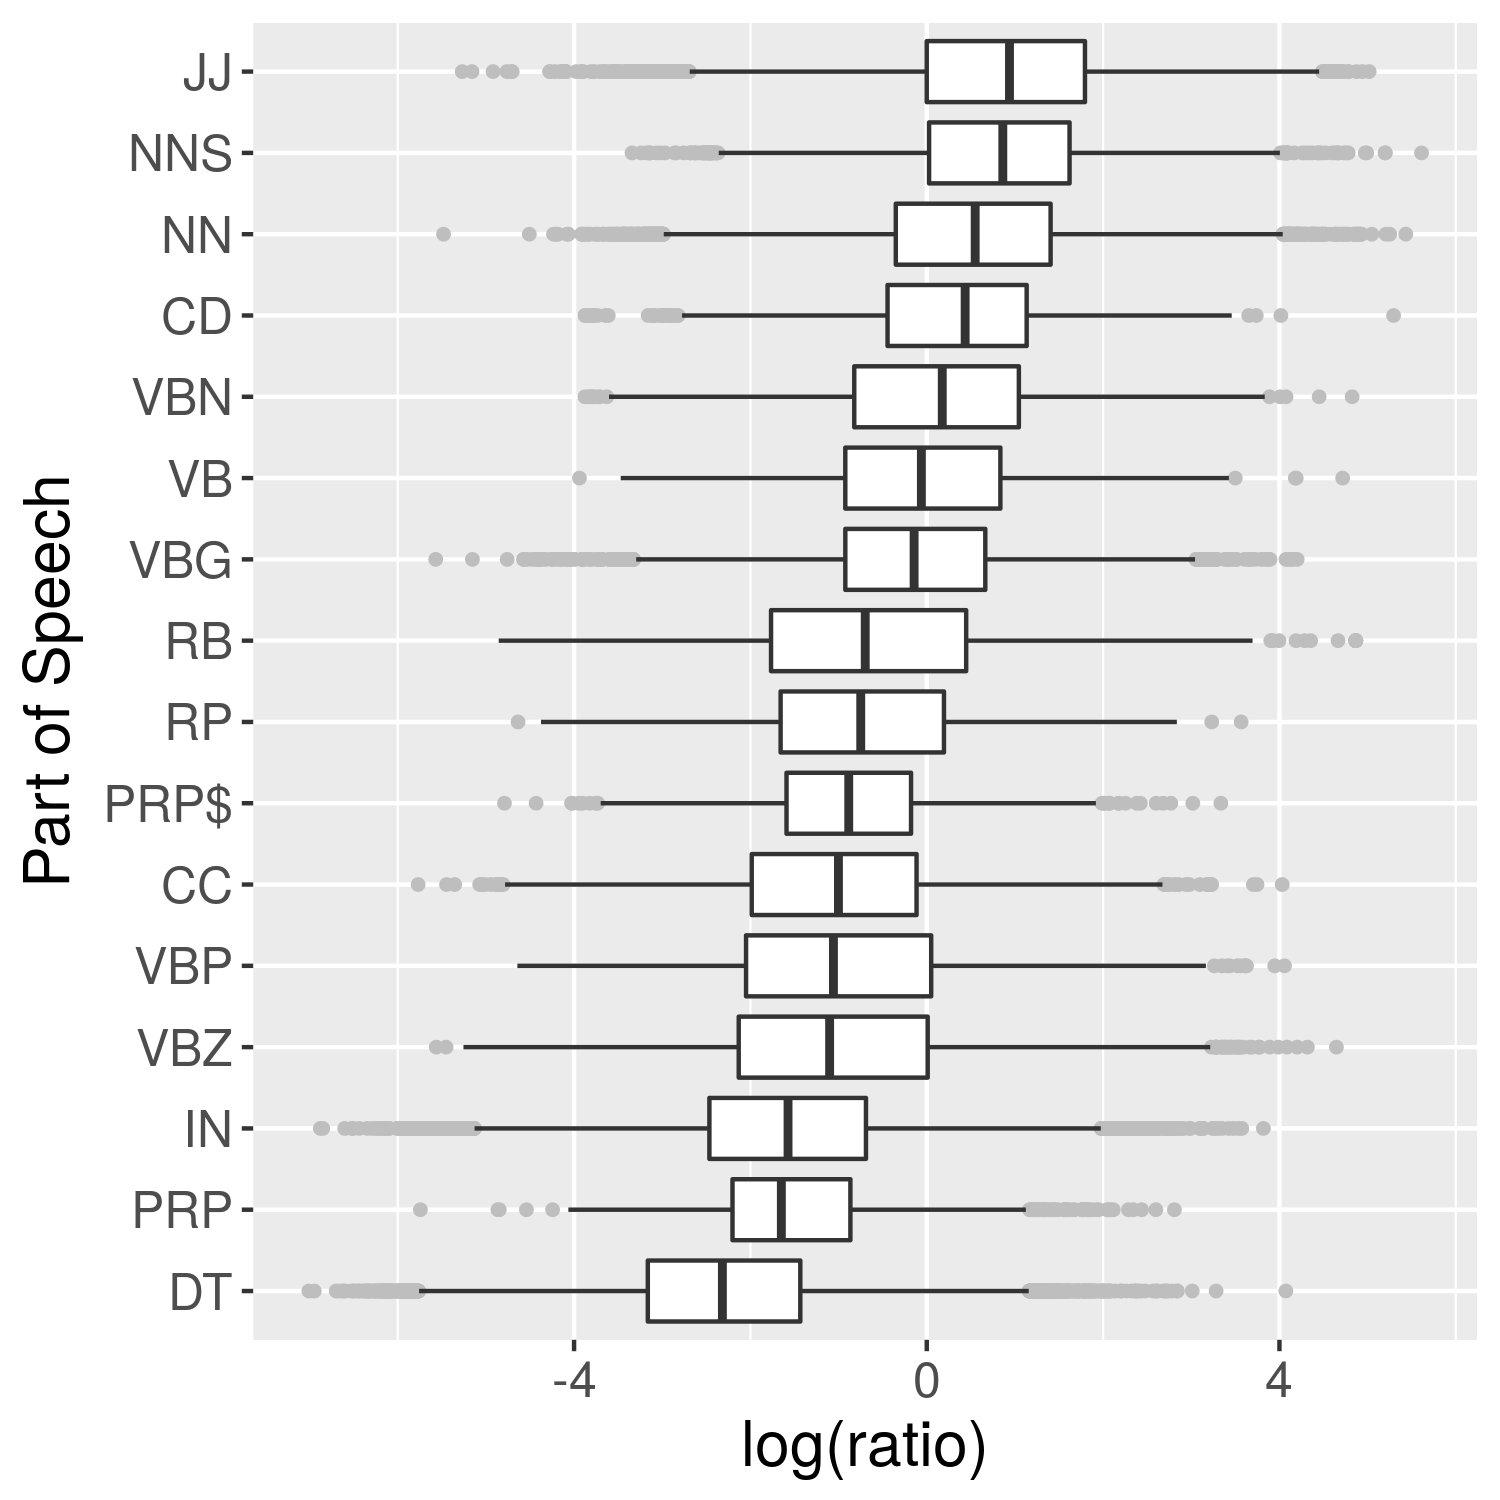
\includegraphics[scale=0.45]{chapters/COLI/imaginet-omission-ratio-pos-boxplot.png} &
  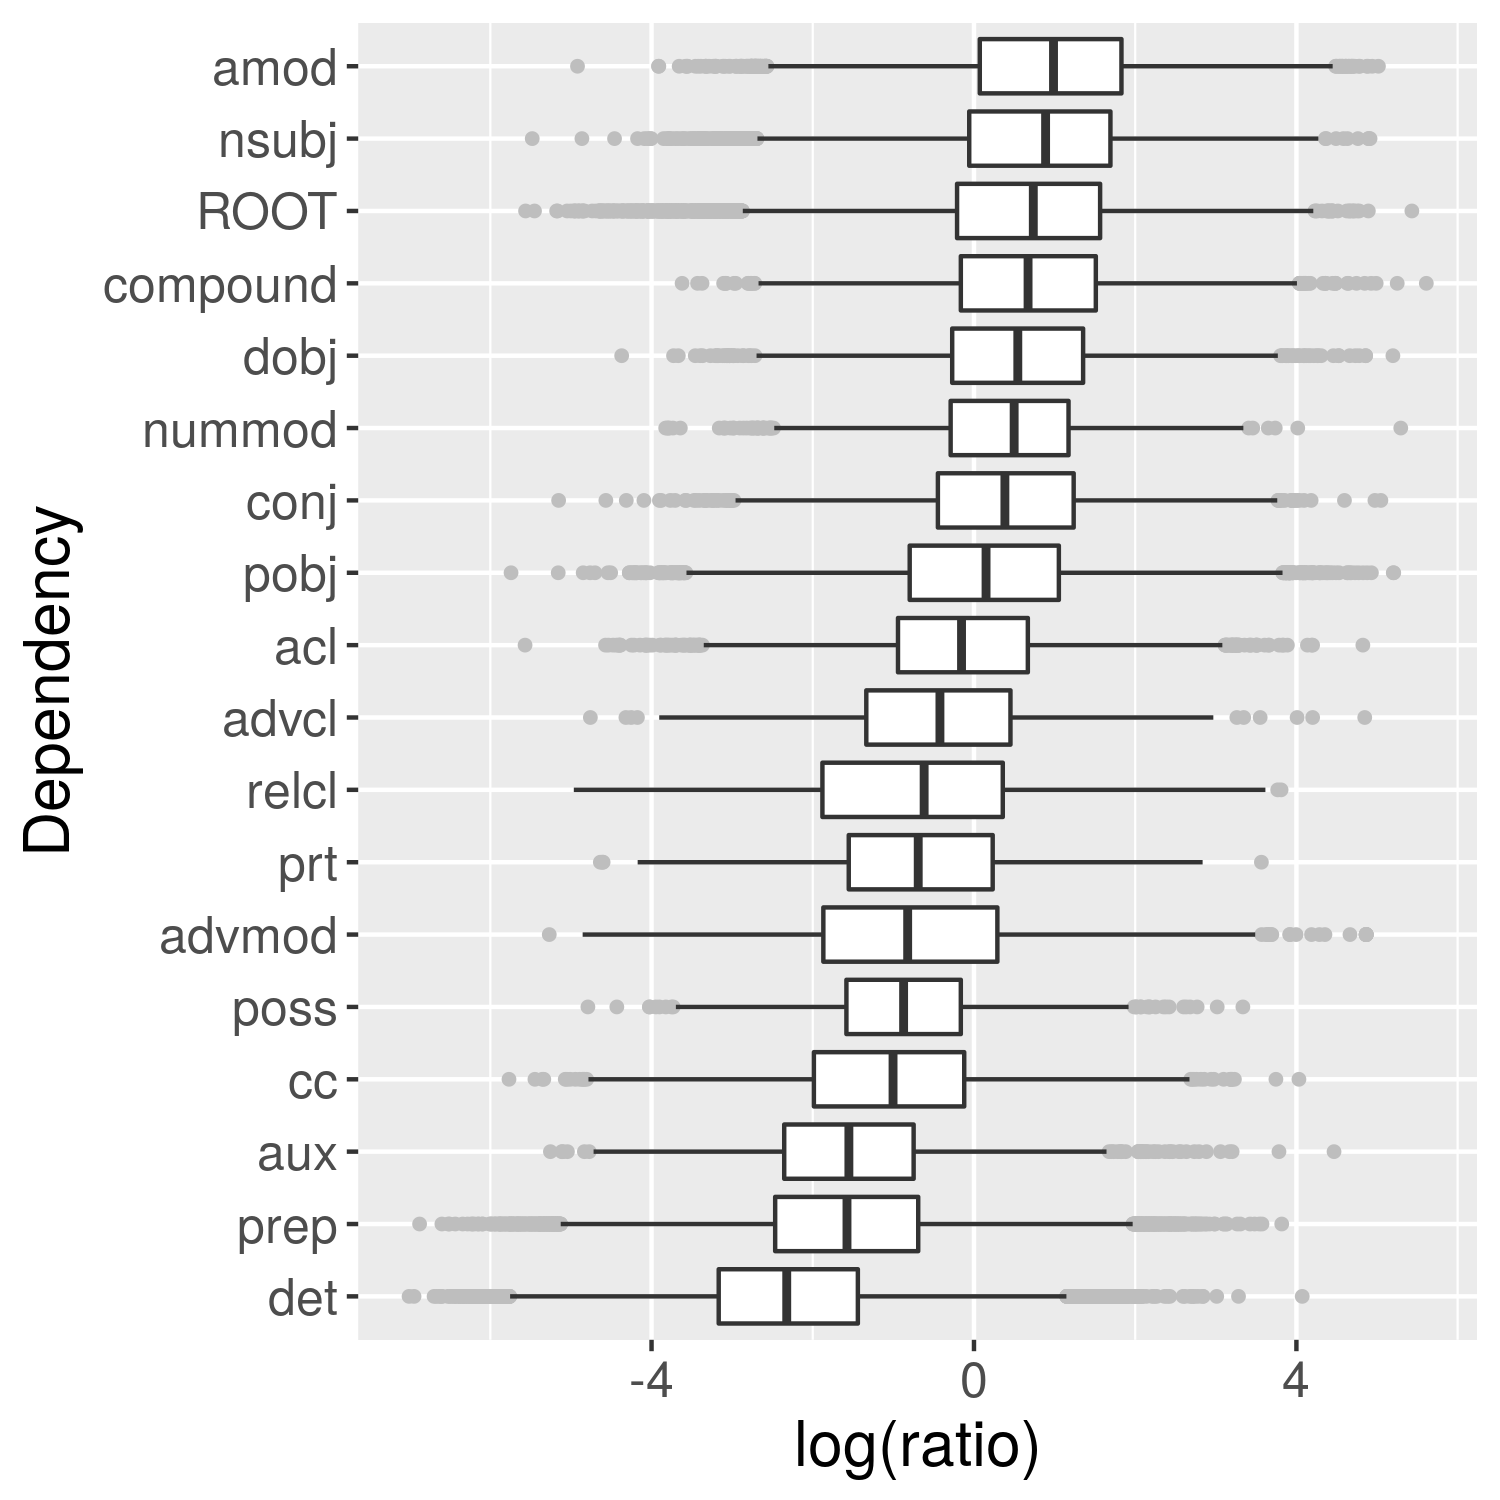
\includegraphics[scale=0.45]{chapters/COLI/imaginet-omission-ratio-dep-boxplot.png} \\
  \end{tabular}
  \caption{Distributions of log ratios of omission scores of {\sc Textual} to {\sc Visual} per
    POS (left) and dependency labels (right). Only labels which occur at least 1250 times are included.}
\label{fig:omission-imaginet-ratio}
\end{figure*}



The omission scores can be used not only to
estimate the importance of individual words, but also of syntactic
categories. We estimate the salience of each syntactic category by
accumulating the omission scores for all words in that category. We
tag every word in a sentence with the part-of-speech (POS) category
and the dependency relation (deprel) label of its incoming arc. For
example, for the sentence \emph{the black dog}, we get ({\it
  the},~DT,~det),
({\it black},~JJ,~amod), ({\it dog},~NN,~root).
Both POS tagging and dependency parsing are performed
using the  \verb+en_core_web_md+ dependency parser from the Spacy package.\footnote{Available at
  \url{https://spacy.io/}.}



Figure~\ref{fig:omission-imaginet} shows the distribution of omission
scores per POS and dependency label for the two pathways of {\sc
  Imaginet} and for {\sc LM}.\footnote{The boxplots in this and
  subsequent figures are Tukey boxplots and should be interpreted as follows: the box extends
from the 25th to the 75th percentile of the data; the line across the
box is the 50th percentile, while the whiskers extend past the lower
and upper quartile to $1.5\times$
the interquartile range (i.e.\ 75th percentile - 25th percentile); the
points are outliers.\label{ft:boxplots}}  The general trend is that for the {\sc
  Visual} pathway, the omission scores are high for a small subset of
labels - corresponding mostly to nouns, less so for adjectives and
even less for verbs - and low for the rest (mostly function words and
various types of verbs). For {\sc Textual} the differences
are \label{edit:textualomission} smaller, and the pathway seems to be
sensitive to the omission of most types of words.  For {\sc LM} the
distribution over categories is also relatively uniform, but the omission scores are higher
overall than for {\sc Textual}.

Figure~\ref{fig:omission-imaginet-ratio} compares the two pathways of
{\sc Imaginet} directly using the log of the ratio of the {\sc Visual}
to {\sc Textual} omission scores, and plots the distribution of this
ratio for different POS and dependency labels.  Log ratios above zero
indicate stronger association with the {\sc Visual} pathway and below
zero with the {\sc Textual} pathway. We see that in relative terms,
{\sc Visual} is more sensitive to adjectives (JJ), nouns (NNS, NN),
numerals (CD) and participles (VBN), and {\sc Textual} to determiners
(DT), pronouns (PRP), prepositions (IN) and finite verbs
(VBZ, VBP).

This picture is complemented by the analysis of the
relative importance of dependency relations: {\sc Visual} pays most
attention to the relations {\sc amod, nsubj, root,
  compound, dobj, nummod}
whereas {\sc Textual} is more sensitive to {\sc det, prep, aux, cc, poss, advmod, prt, relcl}.
As expected, {\sc Visual} is more focused on grammatical
functions typically filled by semantically contentful words, while
{\sc Textual} distributes its attention more uniformly and
attends relatively more to purely grammatical functions.

It is worth noting, however, the relatively low omission scores for verbs in the case
of {\sc Visual}. One might expect that the task of image prediction from
descriptions requires general language understanding and so high omission
scores for all content words in general; however, the results
suggest that this setting is not optimal for learning useful representations of verbs,
which possibly leads to representations that are too task-specific
and not transferable across tasks.

\begin{figure*}[t]
  \centering
  \hspace*{-0.2in}
  \setlength{\tabcolsep}{0pt}
  \begin{tabular}{cc}
  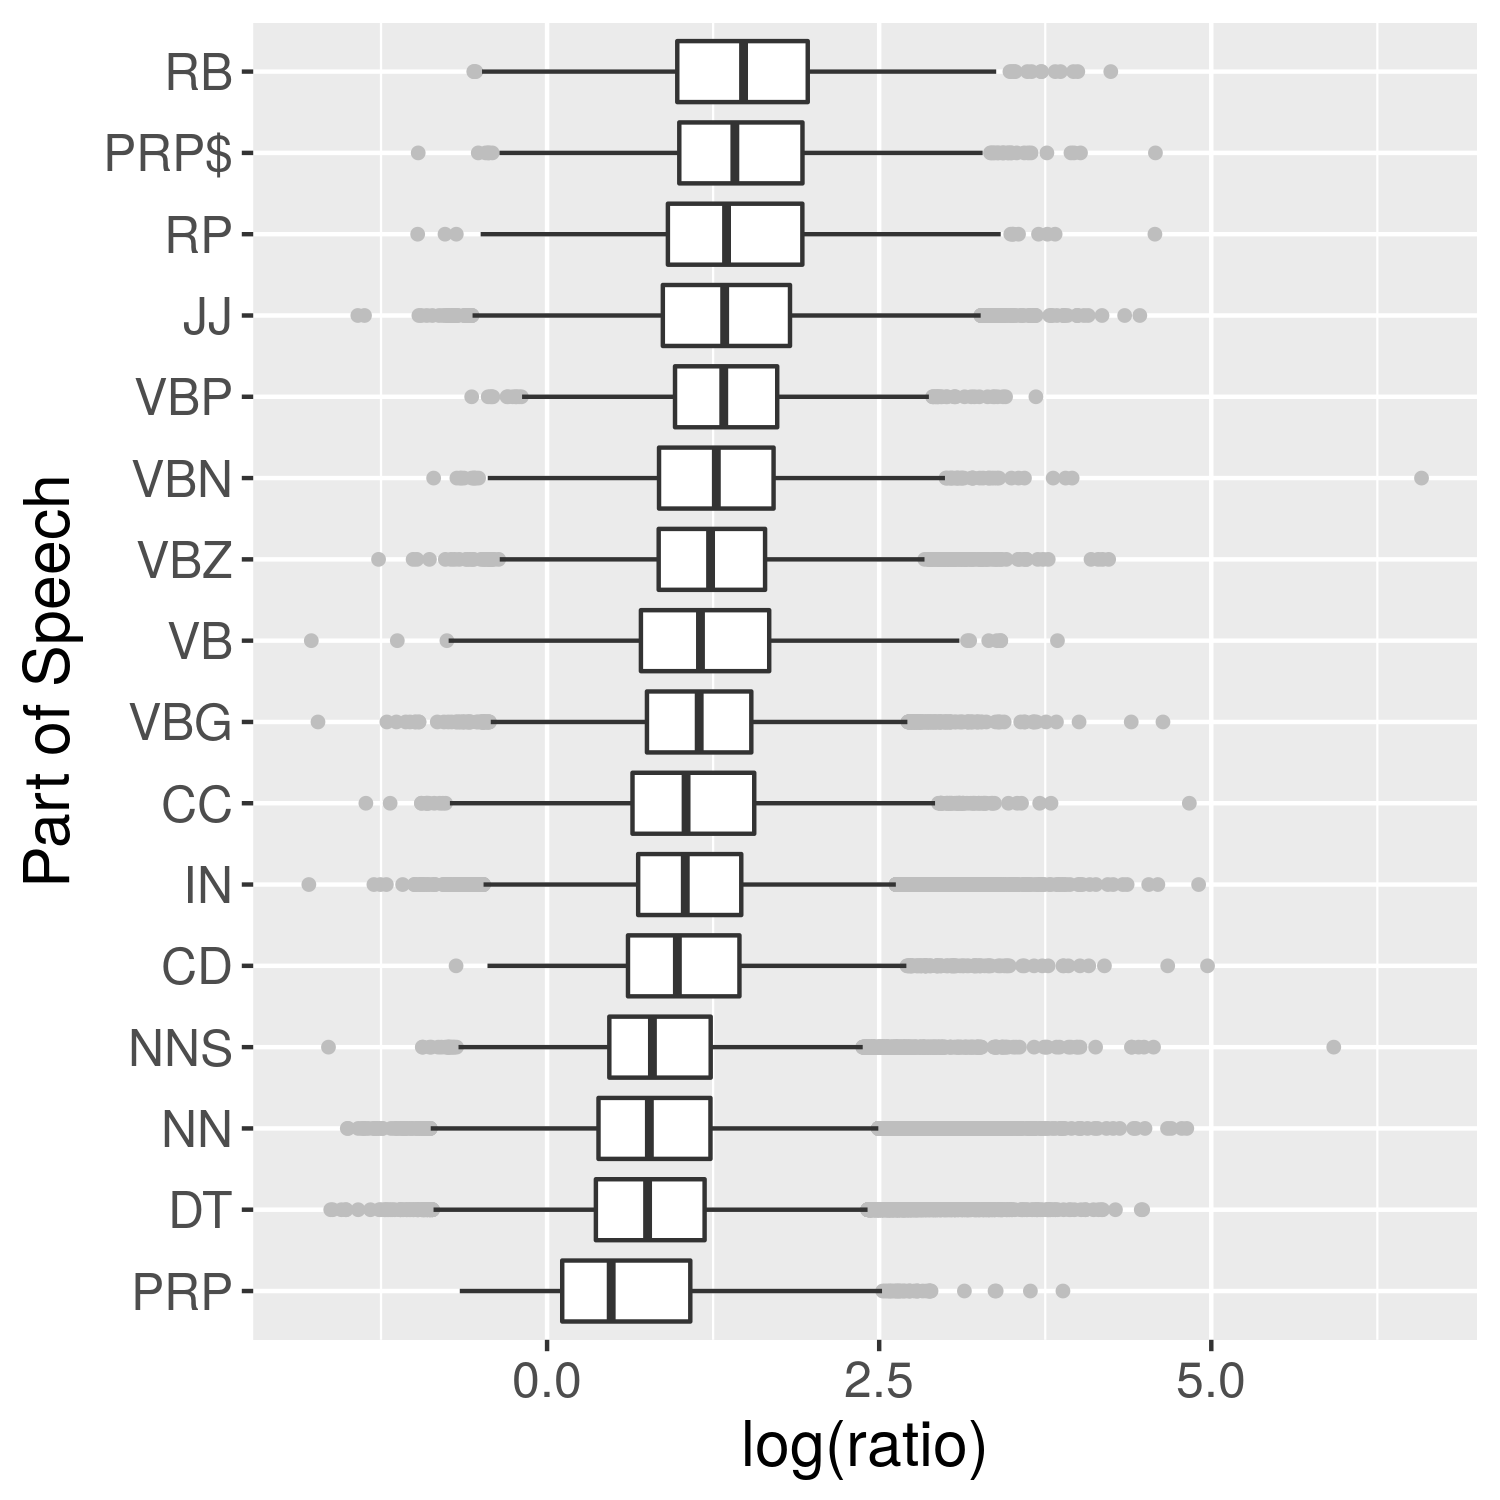
\includegraphics[scale=0.45]{chapters/COLI/imaginet-omission-quotient-pos-boxplot.png} &
  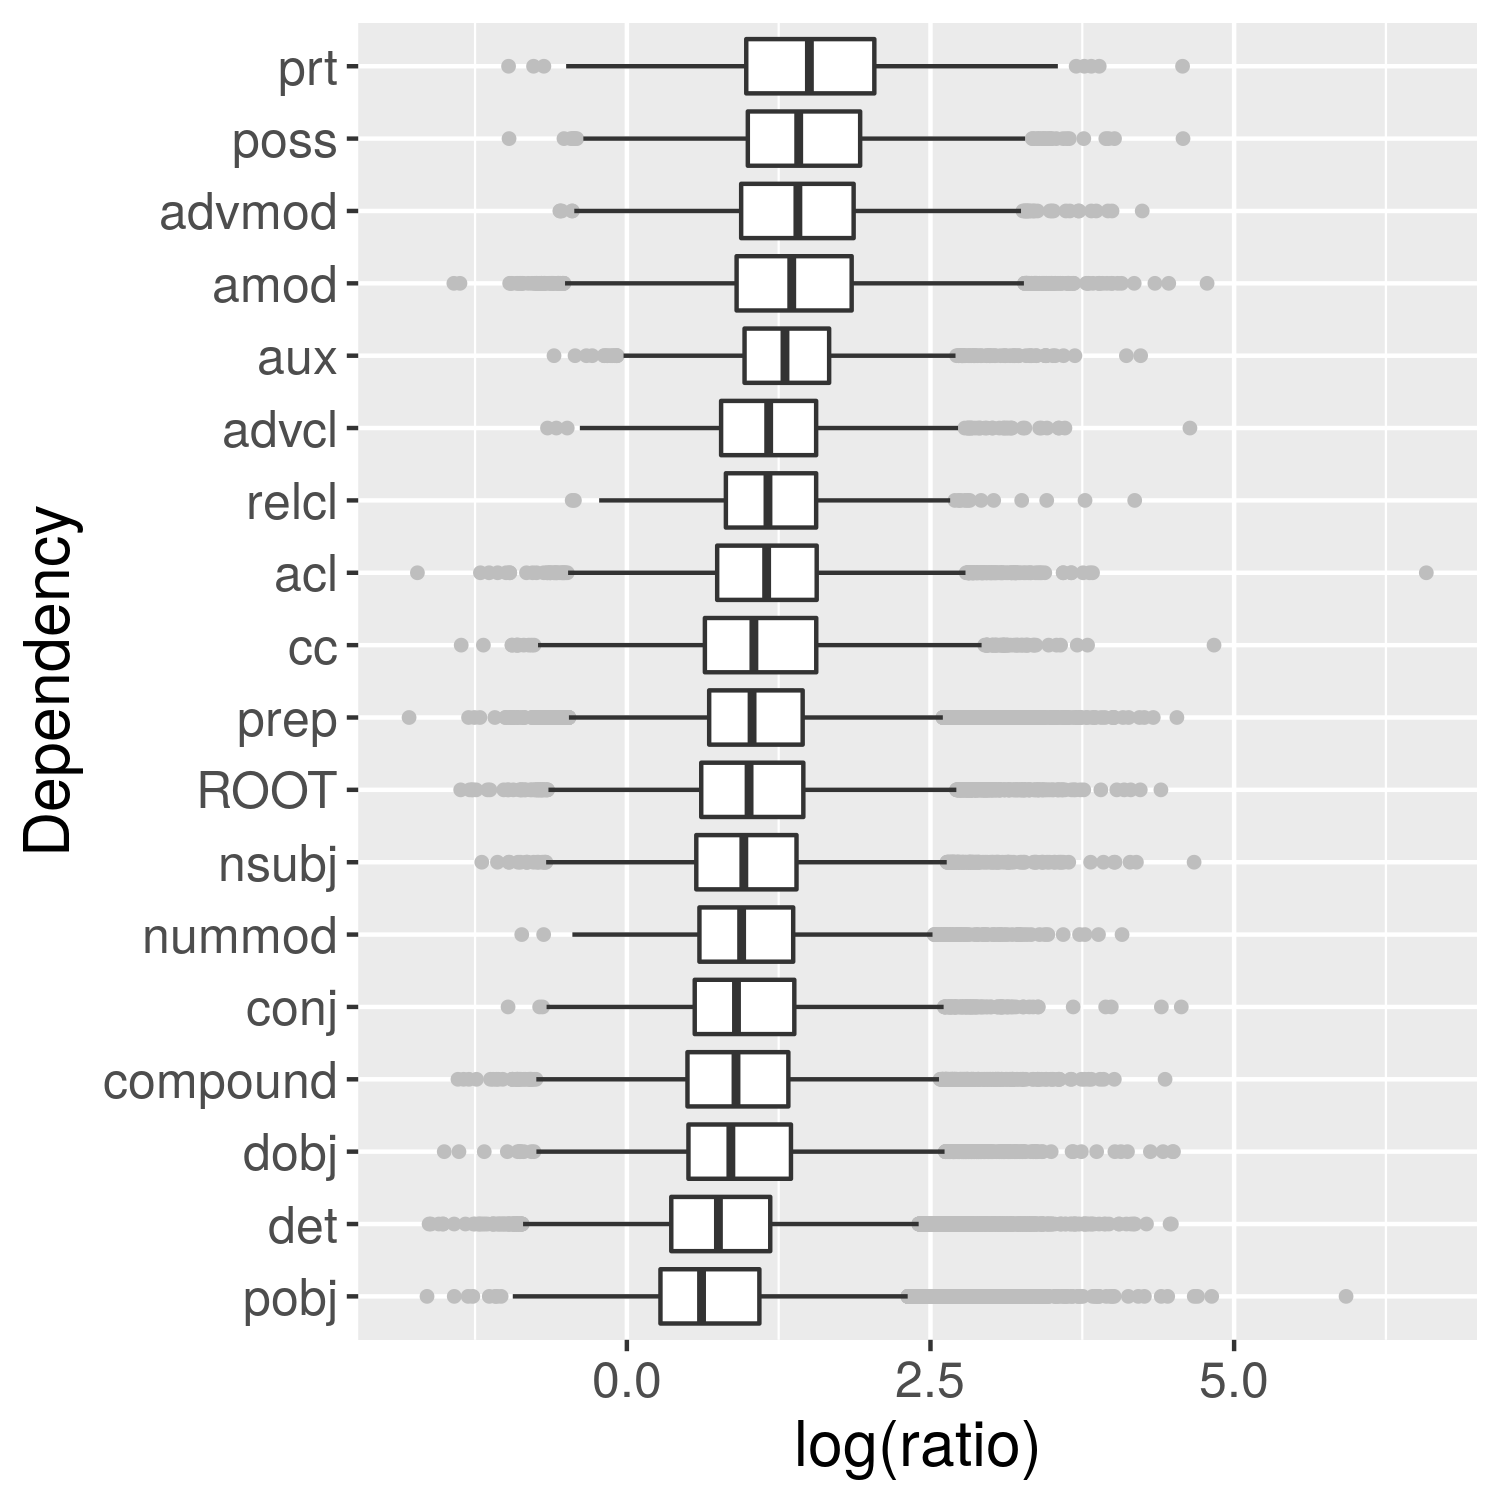
\includegraphics[scale=0.45]{chapters/COLI/imaginet-omission-quotient-dep-boxplot.png} \\
  \end{tabular}
  \caption{Distributions of log ratios of omission scores of {\sc LM} to {\sc Textual} per
    POS (left) and dependency labels (right). Only labels which occur at least 1250 times are included.}
\label{fig:omission-imaginet-quotient}
\end{figure*}


Figure~\ref{fig:omission-imaginet-quotient} shows a similar analysis
contrasting {\sc LM} with the {\sc Textual} pathway of {\sc
  Imaginet}. The first observation is that the range of values of the
log ratios is narrow, indicating that the differences between these
two networks regarding which grammatical categories they are sensitive
to is less pronounced than when comparing {\sc Visual} to {\sc
  Textual}. While the size of the effect is weak, there also seems to
be a tendency for the {\sc Textual} model to pay relatively more
attention to content and less to function words, compared to
{\sc LM}: it may be that the {\sc Visual} pathway pulls {\sc Textual}
in this direction by sharing word embeddings with it.


Most of our findings up to this point conform reasonably well to prior
expectations about effects that  particular learning objectives should
have. This fact serves to validate our methods. In the next section we
go on to investigate less straightforward patterns.


\subsection{Beyond Lexical Cues}
\label{sec:beyondlexical}

Models that utilize the sequential structure of language
have the capacity to interpret the same word type differently depending on
the context. The omission score distributions in Section \ref{sec:omitimaginet}
show that in the case of {\sc Imaginet} the
pathways are differentially sensitive to content vs.\ function
words. In principle, this may be either just due to purely lexical features or the model
may actually learn to pay more attention to the same word type in appropriate
contexts. This section investigates to what extent our models
discriminate between occurrences of a given word in different positions and
grammatical functions.



We fit four L2-penalized linear regression models which predict the omission
scores per token with the following predictor variables:
\begin{enumerate}
	\item {\sc LR word}: word type
	\item {\sc LR +dep}: word type, dependency label and their interaction
	\item {\sc LR +pos}: word type, position (binned as {\sc first, second, third, middle,
	antepenult, penult, last}) and their interaction
	\item {\sc LR full}: word type, dependency label, position, word:dependency interaction,
	word:position interaction
\end{enumerate}

\noindent We use the 5000-image portion of MSCOCO validation data for
training and test. The captions contain about 260,000 words in total, of
which we use 100,000 to fit the regression models. We then use the rest
of the words to compute the proportion of variance explained by the models.
For comparison we also use the {\sc Sum} model which composes word
embeddings via summation, and uses the same loss function as {\sc
  Visual}. This model is unable to encode information about word
order, and thus is a good baseline here as we investigate the
sensitivity of the networks to positional and structural cues.

\begin{table}
  \centering
  \caption{Proportion of variance in omission scores explained by
    linear regression.}
    \begin{tabular}{l|rrrr}
               & word   & +pos  & +dep  & full \\\hline
     {\sc Sum}       & 0.654  & 0.661 & 0.670 & 0.670 \\
     {\sc LM}        & 0.358  & 0.586 & 0.415 & 0.601 \\
     {\sc Textual}   & 0.364  & 0.703 & 0.451 & 0.715 \\
     {\sc Visual}    & 0.490  & 0.506 & 0.515 & 0.523 \\
    \end{tabular}
    \label{tab:lr-r2}
\end{table}


Table~\ref{tab:lr-r2} shows the proportion of variance $R^2$ in omission
scores explained by the linear regression with the different predictors.
The raw $R^2$ scores show that for the language models {\sc LM} and
{\sc Textual}, the word type predicts the omission-score to much smaller
degree compared to {\sc Visual}. Moreover, adding information about
either the position or the dependency labels increases the explained variance for all models.
However, for the {\sc Textual} and {\sc LM} models the position of the word adds
considerable amount of information. This is not surprising considering that the omission
scores are measured with respect to the final activation state, and
given the fact that in a language model the recent history is most
important for accurate prediction.

Figure~\ref{fig:rsquared} offers a different view of the data, showing
the increase or decrease in $R^2$ for the models relative to {\sc LR~+pos}
to emphasise the importance of syntactic structure beyond the position in the sentence.
Interestingly, for the {\sc Visual} model, dependency labels are
more informative than linear position, hinting at the importance of syntactic
structure beyond linear order. There is a sizeable increase in $R^2$ between
{\sc LR~+pos} and {\sc LR~full} in the case of {\sc Visual}, suggesting that
the omission scores for {\sc Visual} depend on the words'
grammatical function in sentences, {\it even after controlling for word
identity and linear position.}  In contrast, adding additional information on
top of lexical features in the case of {\sc Sum} increases the
explained variance only slightly, which is most likely due to the unseen words
in the held out set.

Overall, when regressing on word identities, word position and
dependency labels, the {\sc Visual} model's omission scores are the
hardest to predict of the four models. This suggests that {\sc Visual} may be
encoding additional structural features not captured by these predictors.
We will look more deeply into such potential features in the following sections.

\begin{figure}
\centering
  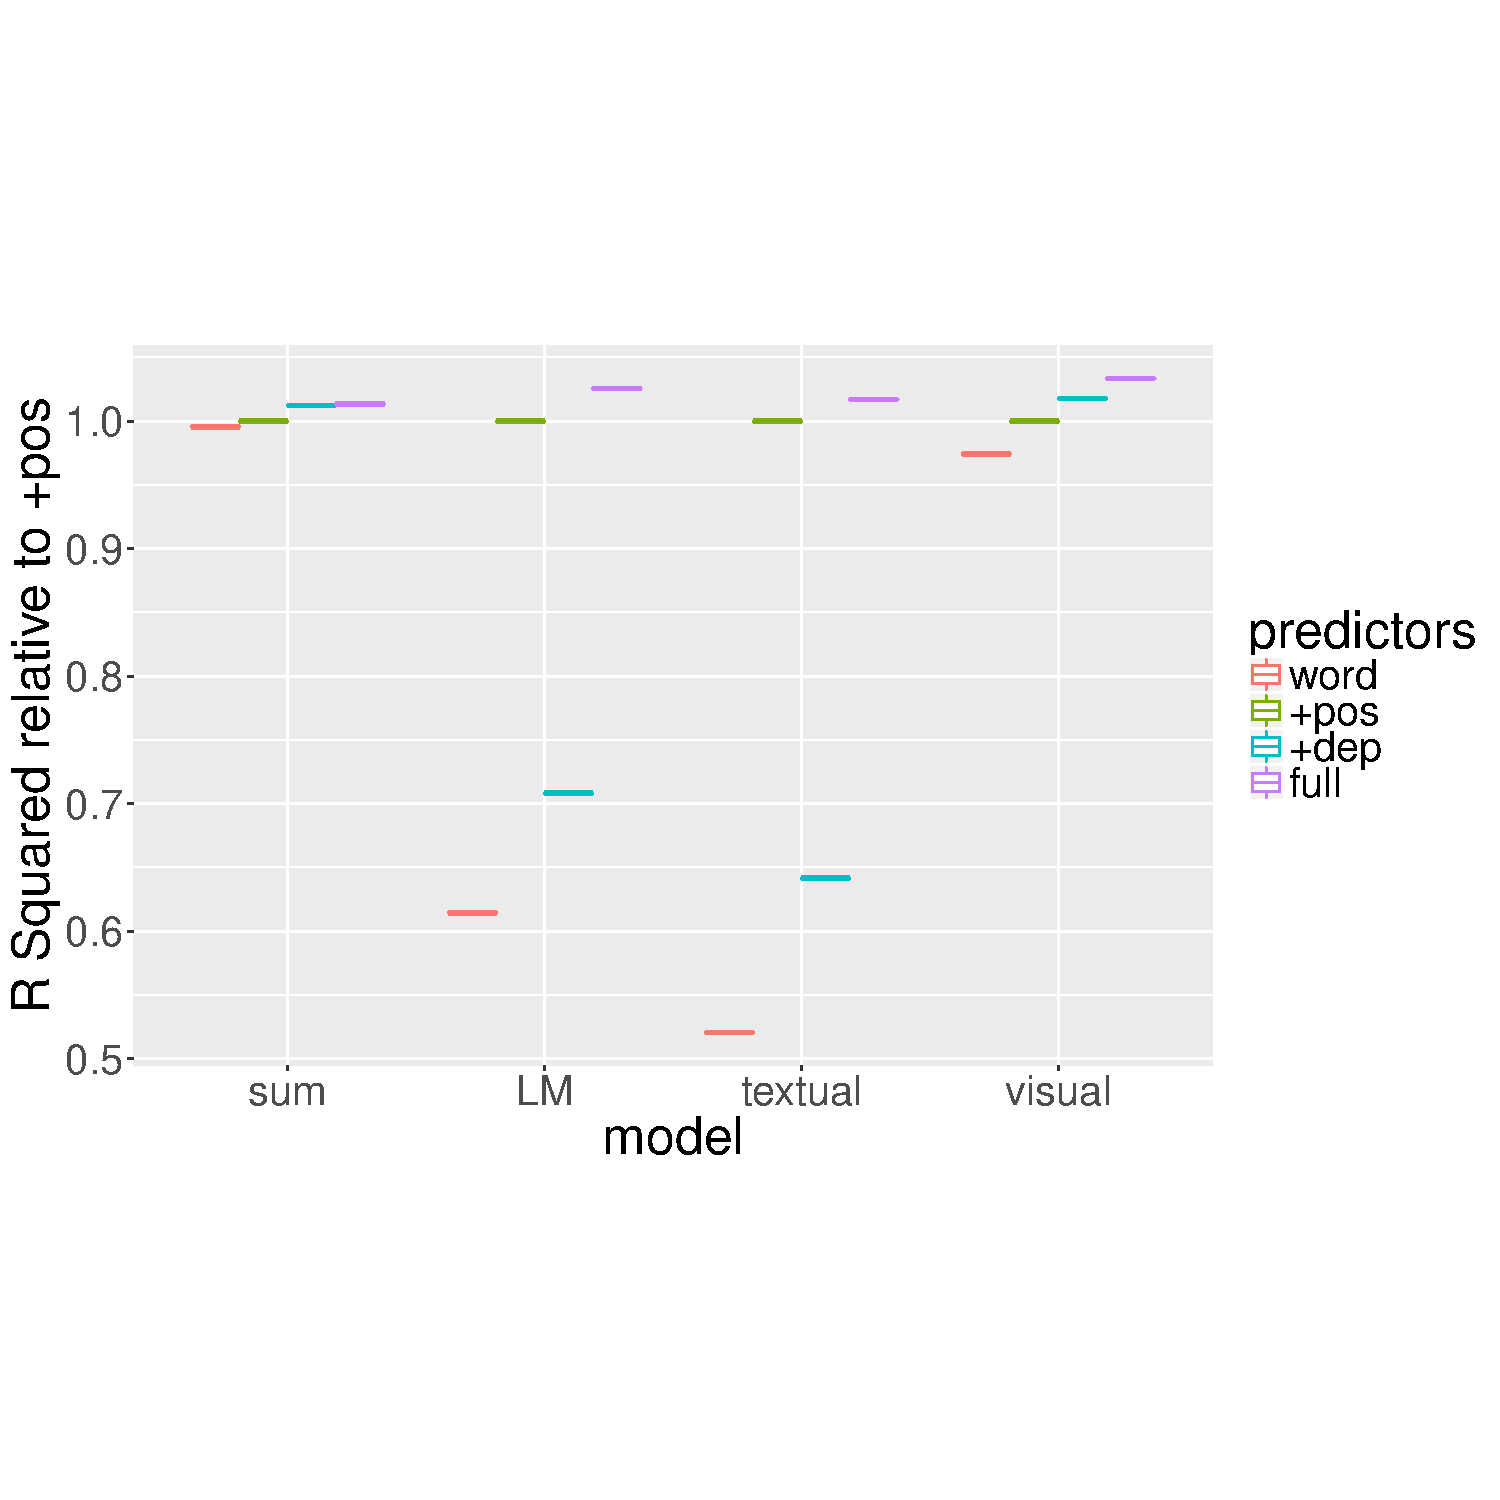
\includegraphics[scale=0.35]{chapters/COLI/position-new.pdf}
\caption{Proportion of variance in omission scores explained by the
  linear regression models
 for {\sc Sum}, {\sc LM}, {\sc Visual} and {\sc Textual}, relative to
 regressing on word identity and position only. }
\label{fig:rsquared}
\end{figure}


\subsubsection{Sensitivity to grammatical function}
\label{sec:gramfunc}

\begin{figure}[t]
  \centering
  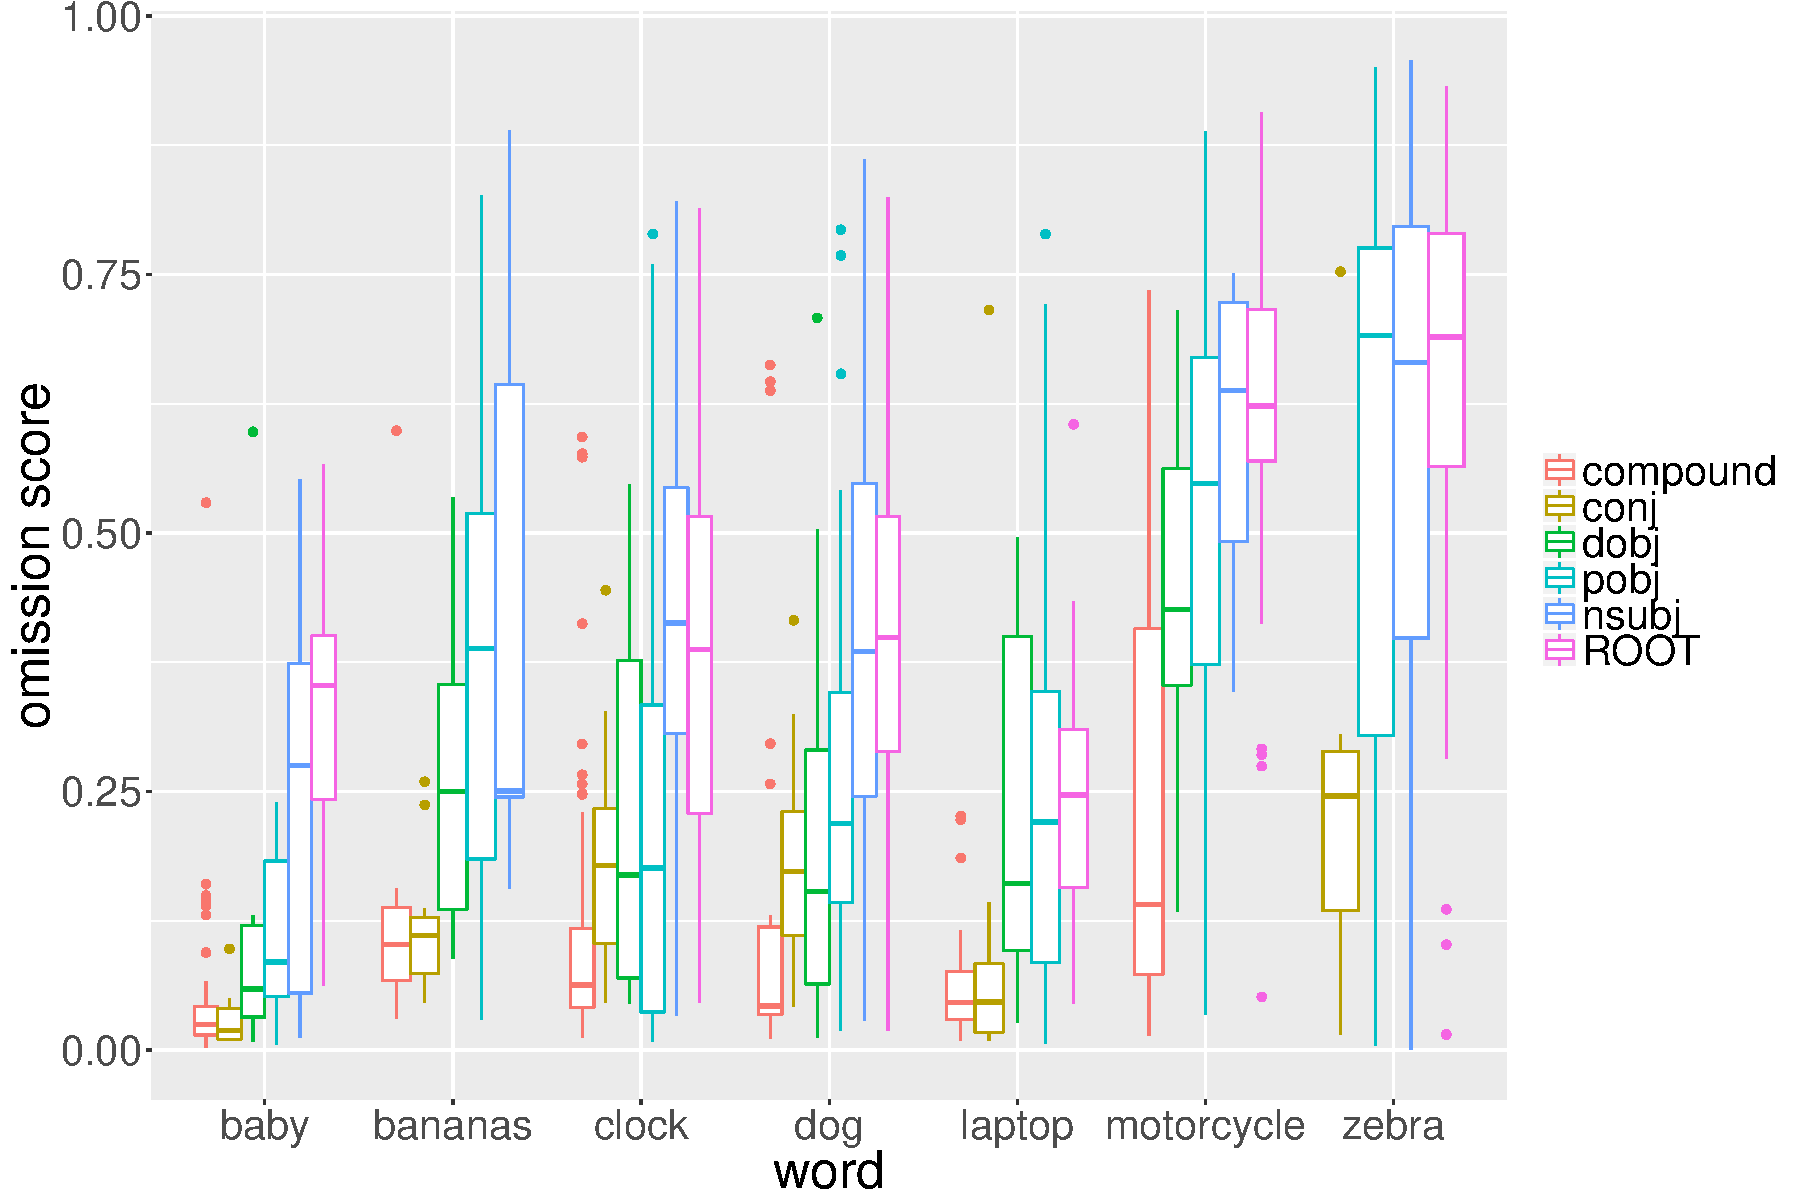
\includegraphics[scale=0.35]{chapters/COLI/top_words.pdf}
  \caption{Distribution of omission scores per dependency label for the selected word types.}
  \label{fig:top_words}
\end{figure}


In order to find out some of the specific syntactic configurations leading to
an increase in $R^2$ between the {\sc LR~word} and {\sc LR~+dep} predictors
in the case of {\sc Visual}, we next considered all word types with
occurrence counts of at least 100 and ranked them according to how much
better, on average, {\sc LR~+dep} predicted their omission scores
compared to {\sc LR~word}.

Figure~\ref{fig:top_words} shows the per-dependency
omission score distributions for seven top-ranked words.
There are clear and large differences in how these words
impact the network's representation depending on what grammatical
function they fulfil. They all have large omission scores when they
occur as {\sc nsubj} (nominal subject) or {\sc root}, likely due to the fact that these
grammatical functions typically have a large contribution to the
complete meaning of a sentence.  Conversely, all have small omission
scores when appearing as {\sc conj} (conjunct): this is probably because in this position
they share their contribution with the first, often more important,
member of the conjunction, for example in {\it A cow and its baby eating
  grass}.

\subsubsection{Sensitivity to linear structure}
\label{subsec:information-struct}

\begin{figure}
\centering
 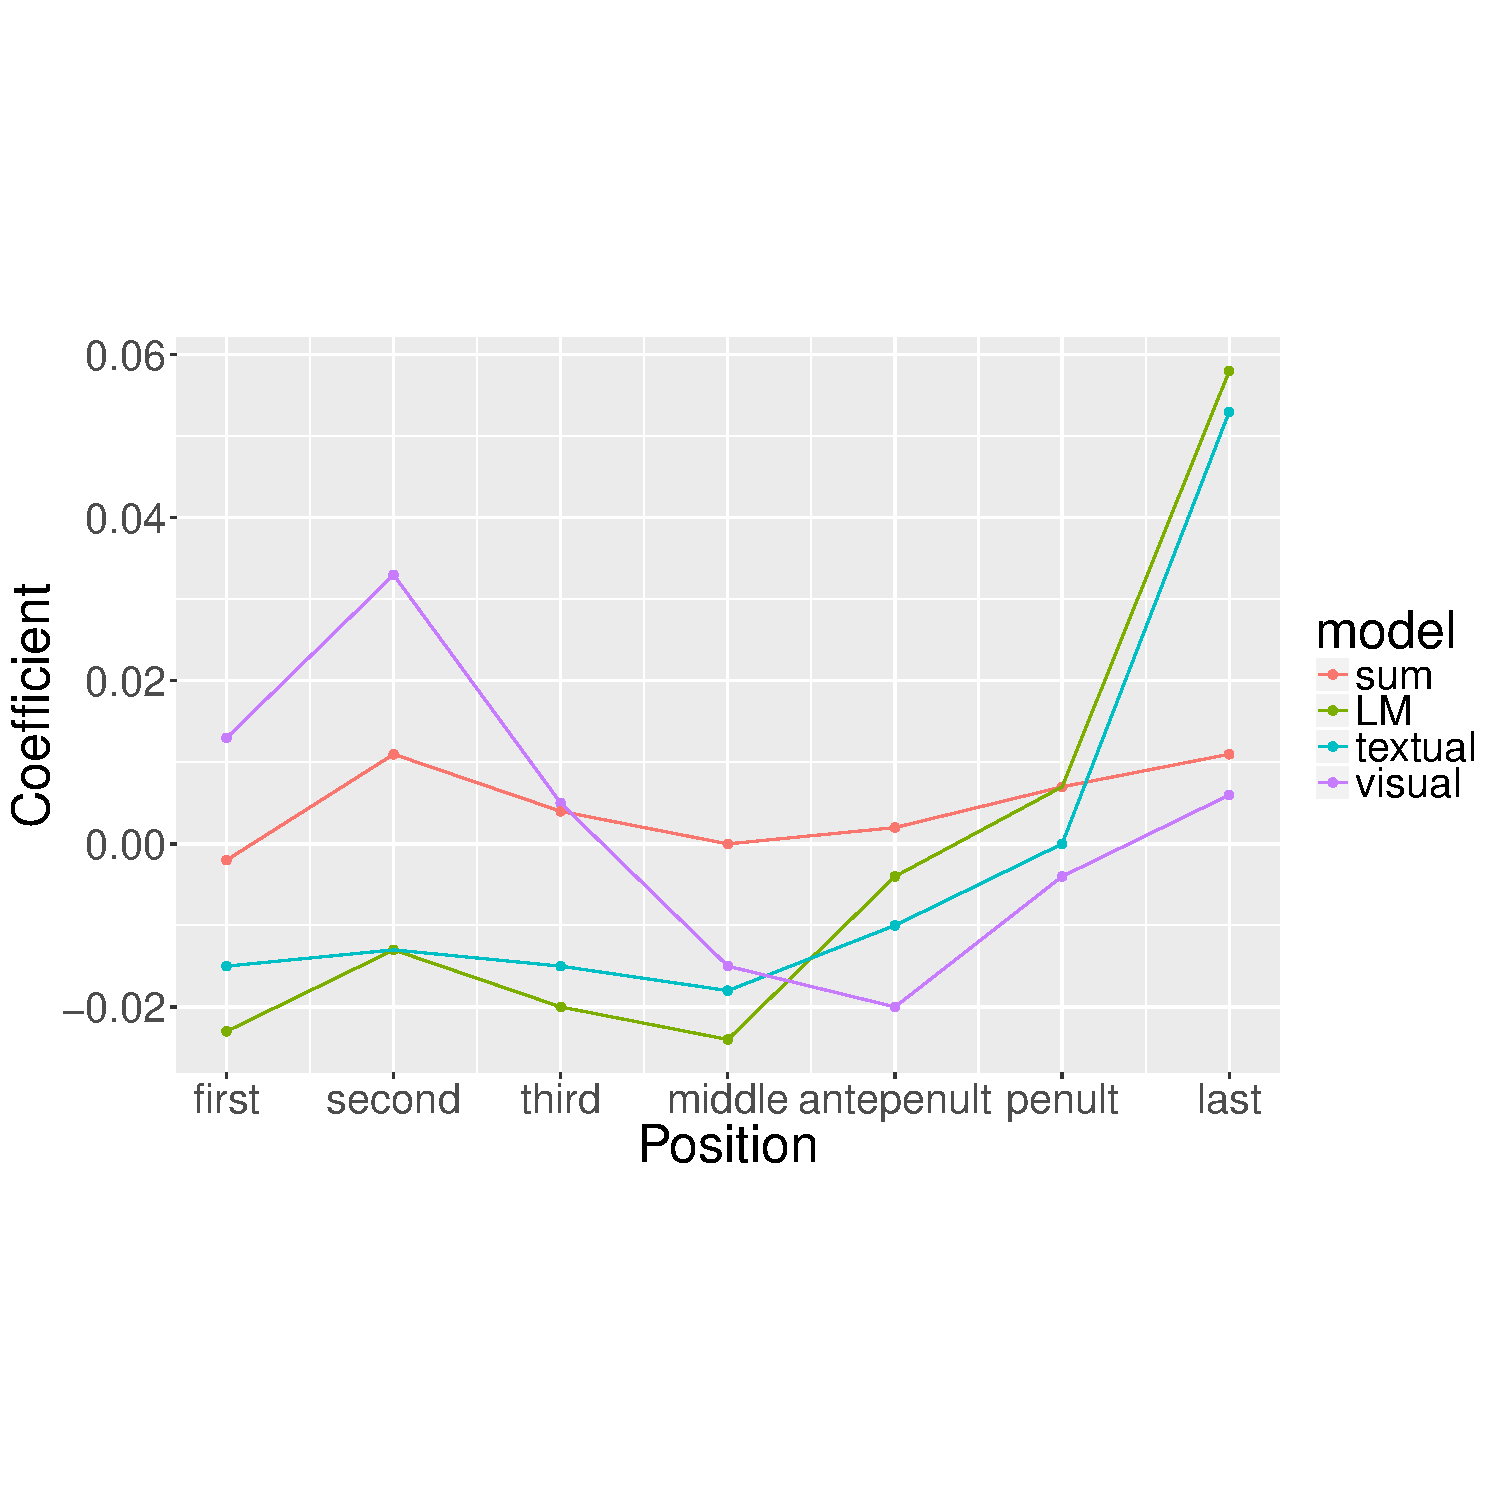
\includegraphics[scale=0.4]{chapters/COLI/position-coef.pdf}
 \vspace{-2cm}
 \caption{Coefficients on the y-axis of {\sc LR full} corresponding to the
position variables on the x-axis.}
 \label{fig:posrqs}
\end{figure}

As observed in Section \ref{sec:beyondlexical},
adding extra information about the position of words
explains more of the variance in the case of {\sc Visual} and especially
{\sc Textual} and {\sc LM}.
Figure \ref{fig:posrqs} shows the coefficients corresponding to the
position variables in {\sc LR~full}. Since the omission scores
are measured at the end-of-sentence token, the expectation is that
for {\sc Textual} and {\sc LM}, as language models,
the words appearing closer to the end of the sentence would have a
stronger effect on the omission scores. This seems to be confirmed by
the plot as the coefficients for these two networks up until the
\emph{antepenult} are all negative.


For the {\sc Visual} model it is less clear what to
expect: on the one hand due to their chain structure,
RNNs are better at keeping track of
short-distance rather than long-distance dependencies and thus we can expect
tokens in positions closer to the end of the sentence to be more important.
On the other hand, in English the information structure of a single
sentence is expressed via linear ordering: the {\sc topic} of a
sentence appears sentence-initially, and the {\sc comment} follows.
In the context of other text types such as dialog or multi-sentence \label{edit:topiccomment}
narrative structure, we would expect {\sc comment} to often be more
important than {\sc topic} as {\sc comment} will often
contain new information in these cases. In our setting of image captions
however, sentences are not part of a larger discourse; it is sentence
initial material that typically contains the most important
objects depicted in the image, e.g. {\it {\underline{two zebras}} are grazing in tall grass on a savannah.}
Thus, for the task of predicting features of the visual scene, it would
be advantageous to detect the topic of the sentence and up-weight its
importance in the final meaning representation. Figure \ref{fig:posrqs}
appears to support this hypothesis and the network does
learn to pay more attention to  words appearing
sentence-initially. This effect seems to be to some extent mixed with the recency
bias of RNNs as perhaps indicated by the relatively high coefficient of the {\it last}
position for {\sc Visual}.

%
\subsection{Lexical versus abstract contexts}
\label{sec:contexts}

We would like to further analyze the kinds of linguistic features that the
hidden dimensions of RNNs encode. Previous work
\cite{karpathy2015visualizing,li2015convergent} has shown that in response
to the task the networks are trained for, individual dimensions in the hidden layers of
RNNs can become {\it specialised} in responding to certain types of triggers, including
the tokens or token types at each time step, as well as the preceding context of
each token in the input sentence.

Here we perform a further comparison between the models based on the hypothesis
that due to their different objectives, the activations of the dimensions of the last
hidden layer of {\sc Visual} are more characterized by semantic relations within
contexts, whereas the hidden dimensions in {\sc Textual} and {\sc LM} are
more focused on extracting syntactic patterns. In order to quantitatively test this
hypothesis, we measure the strength of association between activations of hidden
dimensions and either lexical (token n-grams) or structural (dependency label n-grams) types
of context.

For each pathway, we define $A_i$ as a discrete random variable corresponding
to a binned activation over time steps at hidden dimension $i$, and $C$
as a discrete random variable indicating the context
(where $C$ can be of type `word trigram' or `dependency label bigram', for example).
The strength of association between $A_i$ and $C$ can be measured
by their mutual information:
\begin{equation}
\mathrm{I}(A_i;C) = \sum_{a\in{A_i}}\sum_{c\in{C}} p(a,c)\log\left(\frac{p(a,c)}{p(a)p(c)}\right)
\end{equation}
Similarly to \citep{li2015convergent}, the activation value
distributions are discretized into percentile bins per dimension, such
that each bin contains 5\% of the marginal density. For context types,
we used unigrams, bigrams and trigrams of both dependency labels and
words. Figure~\ref{fig:raw_mutual} shows the distributions of the
mutual information scores for the three networks and the six context
types. Note that the scores are not easily comparable between context
types, due the different support of the distributions; they are,
however, comparable across the networks. The figure shows {\sc LM} and
{\sc Textual} as being very similar, while {\sc Visual} exhibits a
different distribution. We next compare the models' scores pairwise to
pinpoint the nature of the differences.
\begin{figure}
  \centering
  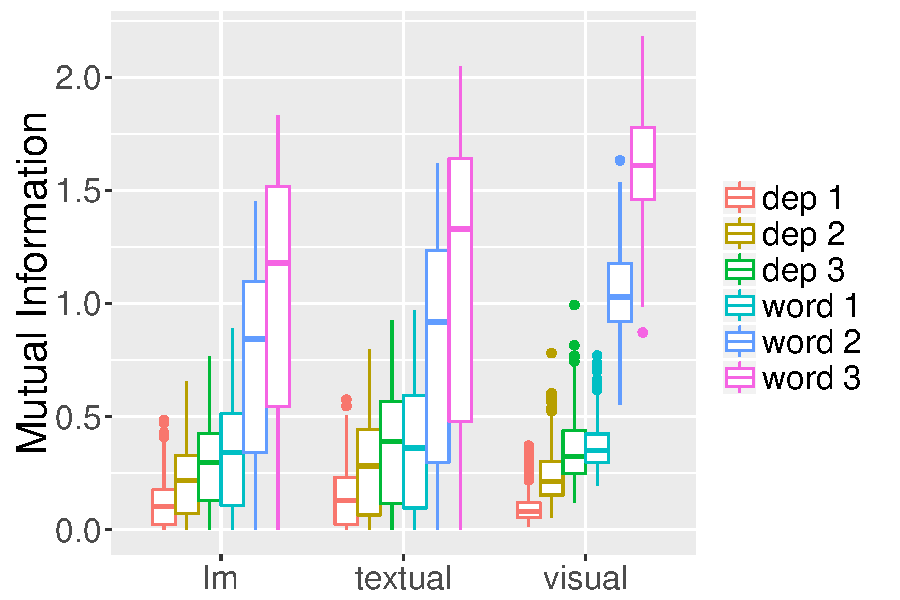
\includegraphics[scale=0.6]{chapters/COLI/raw_mutual.pdf}
  \caption{Distributions of the mutual information scores for the three networks and the six context types.}
  \label{fig:raw_mutual}
\end{figure}

We use the notation $\mathrm{MI}^\mathit{LM}_C$,  $\mathrm{MI}^T_C$ and  $\mathrm{MI}^V_C$
to denote the median mutual information score over all dimensions of {\sc LM}, {\sc Textual} and {\sc Visual}
respectively, when considering context $C$.
We then compute log ratios $\log(\mathrm{MI}^{T}_{C}/\mathrm{MI}^{V}_{C})$ and $\log(\mathrm{MI}^\mathit{LM}_{C}/\mathrm{MI}^{T}_{C})$
for all six context types $C$. In order to quantify variability we bootstrap this statistic with
5000 replicates. Figure~\ref{fig:mi-boot} shows the resulting bootstrap distributions
for uni-, bi-, and trigram contexts, in the word and dependency conditions.


The clear pattern is that for {\sc Textual} versus {\sc Visual}, the
log ratios are much higher in the case of the dependency contexts,
with no overlap between the bootstrap distributions. Thus, in general,
the size of the relative difference between {\sc Textual} and {\sc
  Visual} median mutual information score is much more pronounced for
dependency context types.  This suggests that features that are
encoded by the hidden dimensions of the models are indeed different, and
that the features encoded by {\sc Textual} are more associated with
syntactic constructions than in the case of {\sc Visual}. In contrast,
when comparing {\sc LM} with {\sc Textual}, the difference between
context types is much less pronounced, with distributions
overlapping. Though the difference is small, it goes in the direction
of the dimensions of the {\sc Textual} model showing higher
sensitivity towards dependency contexts.

\begin{figure}
  \centering
  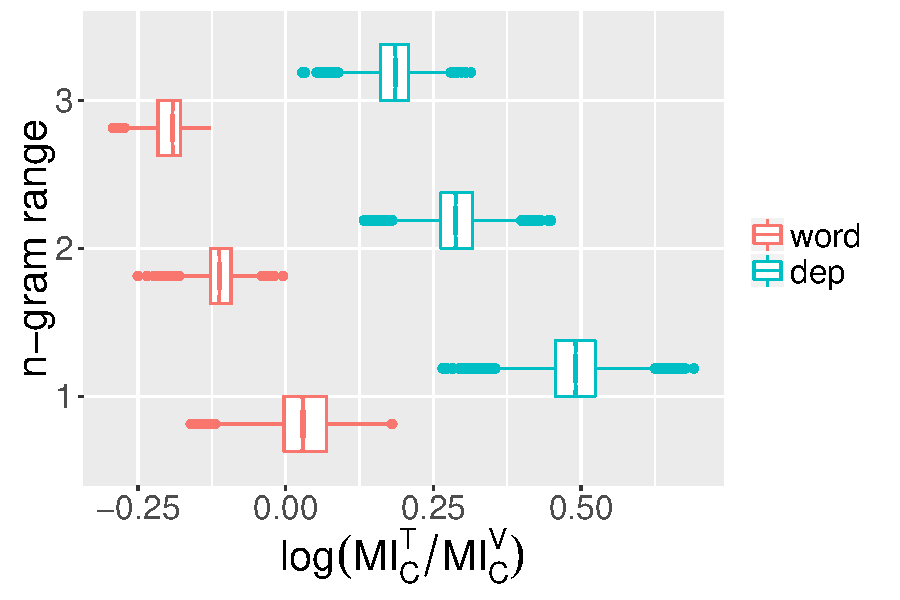
\includegraphics[scale=0.4]{chapters/COLI/bootstrappedMI.pdf}
  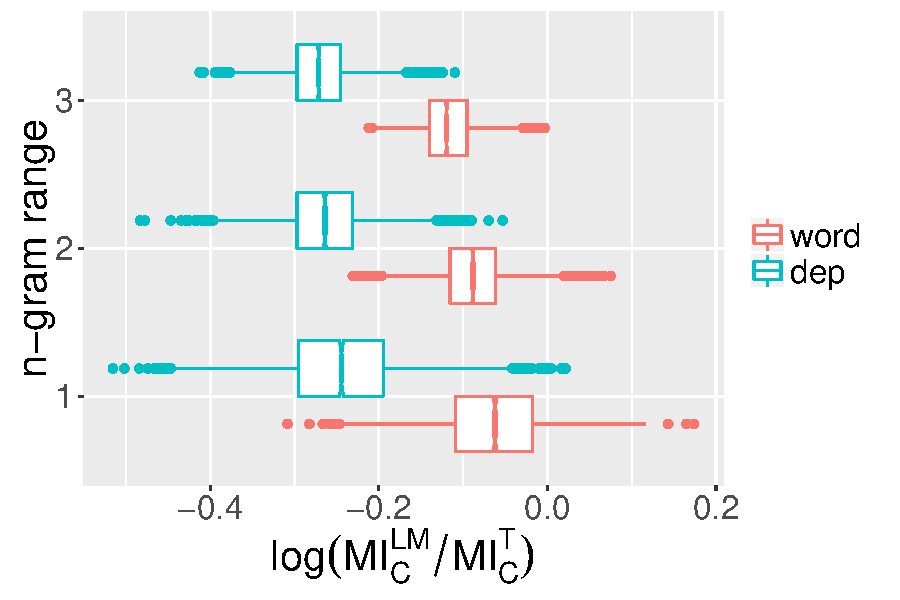
\includegraphics[scale=0.4]{chapters/COLI/bootstrappedMI2.pdf}
  \caption{Bootstrap distributions of log ratios of median mutual
    information scores for word and dependency contexts. Left: {\sc Textual}
      vs {\sc Visual}; right: {\sc LM} vs {\sc Textual}}
  \label{fig:mi-boot}
  \vspace{-.2cm}
\end{figure}


The mutual information scores can be used to pinpoint specific
dimensions of the hidden activation vectors which are strongly
associated with a particular type of
context. Table~\ref{tab:mi-examples} lists for each network the
dimension with the highest mutual information score with respect to
the {\it dependency trigram} context type, together with the top
five contexts where these dimensions carry the highest value. In spite
of the quantitative difference between the networks discussed above,
the dimensions which come up top seem to be capturing something quite
similar for the three networks: (a part of) a construction with an
animate root or subject modified by a participle or a prepositional
phrase, though this is somewhat less clean-cut for the {\sc Visual}
pathway where only two out of five top context clearly conform to this
pattern.  Other interesting templates can be found by visual
inspection of the contexts where high-scoring dimensions are active;
for example, dimension 324 of {\sc LM} is high for {\it word bigram}
contexts including
{\it people preparing, gets ready, man preparing, woman preparing,
  teenager preparing}.

\begin{table}
  \centering
  \caption{Dimensions most strongly associated with the dependency trigram context type, and the top five contexts in which these dimensions have high values.}
\label{tab:mi-examples}
\begin{tabular}{lll}
  Network            & Dimension & Examples         \\\hline
  {\sc LM}           & 511       & cookie/pobj attached/acl to/prep \\
                     &           & people/pobj sitting/acl in/prep \\
                     &           & purses/pobj sitting/pcomp on/prep\\
                     &           & and/cc talks/conj on/prep \\
                     &           & desserts/pobj sitting/acl next/advmod \\\hline
  {\sc Textual}      & 735       & male/root on/prep a/det        \\
                     &           & person/nsubj rides/root a/det   \\
                     &           & man/root carrying/acl a/det \\
                     &           & man/root on/prep a/det         \\
                     &           & person/root on/prep a/det       \\\hline
  {\sc Visual}       &  875      & man/root riding/acl a/det \\
                     &           & man/root wearing/acl a/det \\
                     &           & is/aux wearing/conj a/det \\
                     &           & a/det post/pobj next/advmod \\
                     &           & one/nummod person/nsubj is/aux \\
\end{tabular}
\end{table}

